\chapter{Evolution I}

\section{Introduction to Evolution}

\begin{enumerate}
    \item All living organisms are related through the examination of their DNA sequences. Mass extinctions happened for several times.
    \item Evolution has given rise to huge \textit{diversity}. There are probably more than 10 million species.
    \item Evolution also operates on \textit{massive numbers} of individuals \textit{in parallel}.
\end{enumerate}



\section{Evolution at the molecular level}

\begin{enumerate}
    \item RNA may well have been the first self-replicating molecule to evolve. It is capable of more interesting chemistry and has \textit{lower stability} than DNA.
    \item The greater stability of DNA makes it more suitable for the storage and transmission of information between \textit{generations}.
\end{enumerate}



\section{Quiz 1: Combination of mutated genes}

\bd{Question set}\\[.1in]
An organism divides to make two daughters. Different granddaughters (red, blue) acquire different (rare) mutations that let them and their children grow faster. Perhaps the combination will be even better! Given the random nature of mutations it would take too long for the double mutant to arise by chance. Life has evolved to evolve quickly. What must be going on? Simple and complex organisms have different solutions. \\[.2in]
\bd{Answer}\\[.1in]
As shown, DNA is transferred vertically from parent to child. In order that the different mutations (red, blue) can be combined in one organism there must be some kind of \textit{horizontal transfer} of DNA sequences.
\begin{enumerate}
    \item \bd{Simple organism: Horizontal gene transfer}\\ In prokaryotes\footnote{Prokaryotes are unicellular organisms that lack organelles or other internal membrane-bound structures.}, such horizontal gene transfer is mediated by several mechanisms (conjugation\footnote{A specific mechanism to transfer DNA between cells. The basis for much antibiotic resistance, which can be transferred quite efficiently.}, transduction\footnote{Viruses pick up and move random host genes to new cells.}, transformation\footnote{Random uptake of DNA from the environment} or molecular bioenineering). These transfers tend to involve \udl{transfers} of short lengths of DNA (compared to the total length of the chromosome), and can be random and infrequent.
    
   \item \bd{Complex organism: Sexual reproduction}\\ In complex organisms, \udl{sexual reproduction} allows an extremely efficient mixing of DNA as each child receives a single complement of genetic information ($n$ chromosomes) from each parent ($2n$). Furthermore, the parental chromosome pairs line up and recombine before being passed on, so that a new combination of variations is passed on.
\end{enumerate}


\section{Evolutionary and phylogenetic trees}

\begin{enumerate}
    \item \bd{Prokaryotes} Prokaryotes have no membrane-surrounded nucleus containing DNA, as the eukaryotes do.
    \begin{enumerate}
        \item \bd{Archaea} Archaea include most of the extremophiles but also methane-generating gut bacteria.
        \item \bd{Bacteria}
    \end{enumerate}
    \item \bd{Eukaryotes} Eukaryotes have \udl{cells} with \udl{complex} internal structures and include all the Eukaryotes plants and animals but also microbes e.g. yeast\footnote{A type of fungus commonly used for alcoholic beverages and baking.}. The original eukaryotes are likely to have formed through a symbiosis between archeal and bacterial cells.
\end{enumerate}


\section{A View of Darwinian evolution}

\begin{figure}[h]
\centering
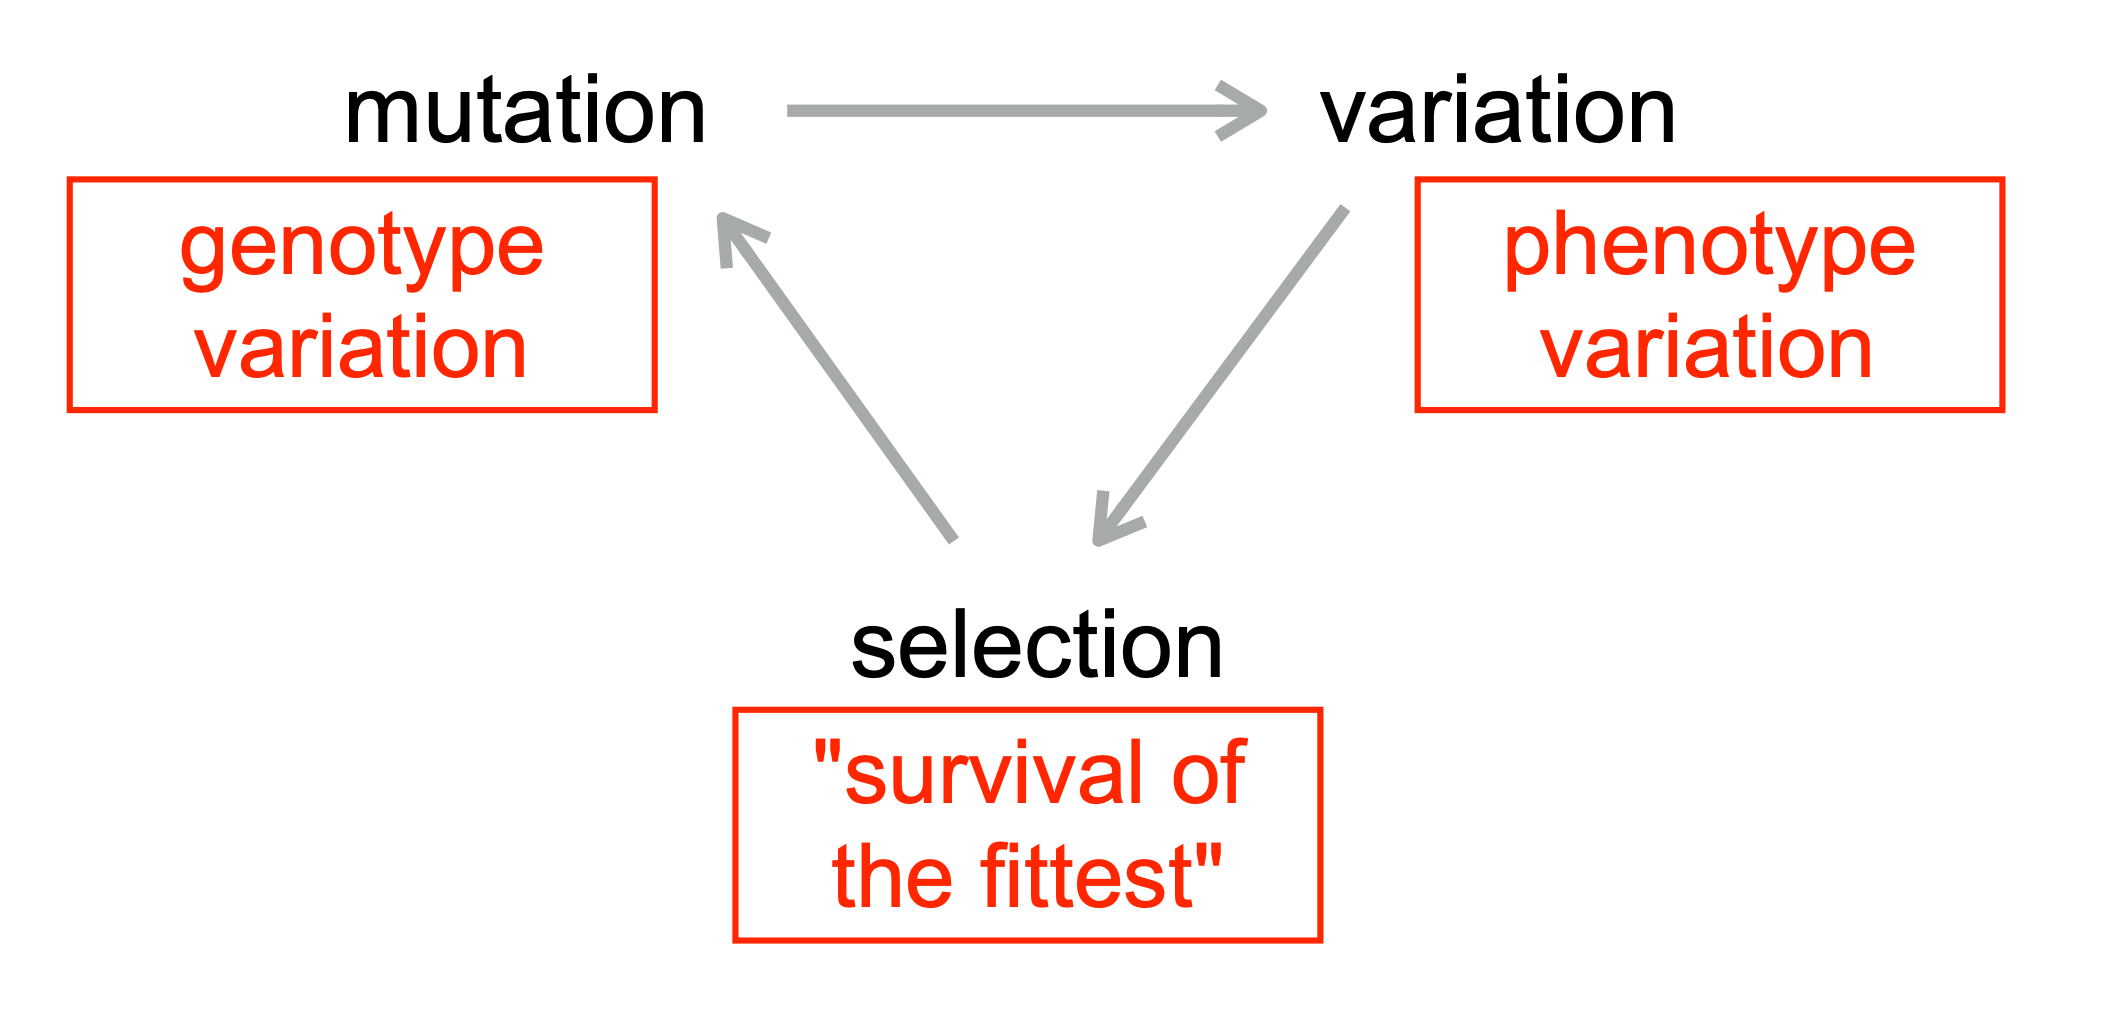
\includegraphics[width=1\textwidth]{images/lecture1.png}\\[.2in]
\caption{A View of Darwinian evolution} 
\end{figure}


\section{Quiz 2: Interfere evolution}
Given the Darwinian evolution graph, where can we interfere?
\begin{enumerate}
    \item \bd{mutation}: random mutagenesis, design specific mutations or introduce new functions.
    \item \bd{phenotypic variation}: conducive environment.
    \item \bd{selection}: artificial selection.
\end{enumerate}